\documentclass[11pt, letterpaper]{article}
\usepackage{graphicx} % Required for inserting images

\usepackage[margin=1.1in]{geometry}
\usepackage{amsmath, amssymb, amsthm}
\usepackage{booktabs}
\usepackage{array}
\usepackage{hyperref}
\usepackage{xcolor}
\usepackage{graphicx}
\usepackage{caption}
\usepackage{subcaption}
\usepackage{parskip}
\usepackage{microtype}
\usepackage{enumitem}
\usepackage[explicit]{titlesec}

\hypersetup{
  colorlinks = true,
  linkcolor  = blue!60!black,
  citecolor  = blue!60!black,
  urlcolor   = blue!60!black,
}

\titleformat{\section}{\large\bfseries}{\thesection.}{0.5em}{#1}[\vspace{-0.3em}\rule{\linewidth}{0.4pt}]
\titleformat{\subsection}{\normalsize\bfseries}{\thesubsection}{0.5em}{#1}

\newcommand{\refsys}{\mathrm{ref}}
\newcommand{\bref}{b_{i,\refsys}}
\newcommand{\refscale}{\mathrm{ref\_scale}}

\newtheorem{lemma}{Lemma}
\newtheorem{proposition}{Proposition}

% ------------------------------------------------------------------ %
\title{\textbf{Notes on sensor array nearest neighbor interaction theory project}\\[0.4em]
  \large Resonant Coupled Oscillator Simulator \\
  Physics, Optimization, and Results}
\author{George Issa, Nancy Aggarwal, Richard Scalettar}
\date{\today}
% ------------------------------------------------------------------ %

\begin{document}
\maketitle
\tableofcontents
\newpage

% ================================================================== %
\section{Overview}
% ================================================================== %

\textbf{ResOSc} is a Python package for simulating and analyzing chains of
coupled mechanical oscillators, with direct application to precision physics
experiments such as gravitational-wave (GW) detectors and dark-matter (DM)
sensors.  Given a set of masses $m_i$, wall springs $k_{ii}$, and coupling
springs $k_{i,i+1}$, the package:
\begin{enumerate}[noitemsep]
  \item solves the eigenvalue problem to obtain normal-mode frequencies
        $\omega_i^*$ and eigenvectors;
  \item computes the forced response under a chosen physical driving model;
  \item finds the optimal linear observable (weight vector over oscillator
        readouts) that maximizes worst-case detection sensitivity; and
  \item searches the full parameter space via Monte Carlo to find
        configurations that simultaneously maximize sensitivity and frequency
        coverage.
\end{enumerate}

\subsection{Roadmap: From Dimensionless Theory to a Physical Detector
Forecast}
\label{sec:roadmap}

The results in these notes were first developed in dimensionless units with
an amplitude-based figure of merit.  The programme now underway grounds the
pipeline in the physical framework of the companion note \emph{SNR of a
Multimode Mechanical Detector} and the levitated-sensor detector (LSD)
platform [Aggarwal \emph{et al.}, PRL \textbf{128}, 111101 (2022);
arXiv:2010.13157], targeting the science case of planetary-mass primordial
black hole (PBH) binaries [Miller \emph{et al.}, PRL \textbf{133}, 111401
(2024)] and weakly interacting (``gentle'') dark matter.  The plan:

\begin{enumerate}[noitemsep]
  \item \textbf{Objective.}  Replace the amplitude minimax by the
        matched-filter signal-to-noise ratio
        $\rho^2 = 4\int |\tilde h(f)|^2 / S_h(f)\, df$, reported as a
        \emph{horizon distance} $d_{\max}(\mathcal{M}_c)$ for benchmark PBH
        chirp masses (inspiral spectrum
        $|\tilde h|^2 = \mathcal{A}^2 f^{-7/3}$), and as minimum detectable
        impulse / coupling for the dark-matter channels.  The full
        transfer-function integral treats overlapping resonances exactly,
        retiring the isolated-peak/swept metric dichotomy of
        Sec.~\ref{sec:universal-bound}; the resolvability condition survives
        only as the validity criterion of the per-mode approximation.  The
        broadband source spectrum also subsumes the former ad-hoc
        frequency-spread objective.
  \item \textbf{Noise model.}  Thermal force noise from the
        fluctuation--dissipation theorem
        ($S_F = 4k_BT m_i\gamma_i$, uncorrelated in UHV) plus readout shot
        noise, combined into the strain-referred PSD
        $S_h(f) = S_O^{\mathrm{noise}}(f)/|T(f)|^2$.
  \item \textbf{Two readouts, compared.}  Readout A (axial cavity probe:
        one channel, weights fixed by the intracavity field --- design
        freedom is purely mechanical) and Readout B (transverse imaging:
        $N$ channels, freely optimizable weights and probe-power
        allocation).  Both are computed for every design; thermal- and
        readout-limited regimes are both evaluated, with the crossover
        frequency reported.
  \item \textbf{Units and benchmark.}  SI throughout; the benchmark
        parameter block follows the LSD proposal (stacked SiO$_2$/Si discs,
        $r = 75\,\mu$m, trap frequencies 10--100~kHz,
        $P = 10^{-11}$~Torr, $L = 10$~m cavity, damping
        0.17--1.7~Hz, target $\sqrt{S_h}\sim 10^{-21}$--$10^{-22}\,
        \mathrm{Hz}^{-1/2}$), with unconfirmed entries (disc mass, detected
        powers, quantum efficiency, cavity pole, effective temperature)
        flagged for confirmation.
  \item \textbf{Physical coupling constraints.}  Couplings are
        parameterized by mechanism rather than free box bounds; the first
        implementation uses Coulomb coupling between charged particles
        ($k_{ij} \propto q_i q_j / d_{ij}^3$, long-range tails included),
        whose stray-charge floor gives the coupling-floor constraint of the
        route-3 study its physical origin.  Optical-binding (correlated
        noise) and cavity-mediated (non-symmetric stiffness) couplings are
        documented extensions.
  \item \textbf{Deliverable.}  Sensitivity curves $\sqrt{S_h(f)}$ and PBH
        horizon distances for optimized coupled arrays versus the best
        uncoupled array, under laboratory parameters --- restating the
        coupled-vs-uncoupled questions of these notes in units a lab can
        act on.
\end{enumerate}

\begin{table}[h]
\centering
\caption{The two readout strategies (companion note Sec.~8) and their
consequences for the optimization pipeline.  Both observe the same
resonant motion of the coupled array; they differ in what may be
optimized and in the readout-noise shape.}
\label{tab:readouts}
\begin{tabular}{@{}p{0.24\linewidth}p{0.34\linewidth}p{0.34\linewidth}@{}}
\toprule
 & \textbf{Readout A (cavity)} & \textbf{Readout B (imaging)} \\
\midrule
Geometry & axial cavity probe, $\lambda = 1064$\,nm &
  transverse imaging, $\lambda = 532$\,nm \\
Channels & 1 (one optical phase) & $N$ (one per particle) \\
Weights $w_i$ & \emph{fixed} by the intracavity field,
  $\mathbf{w} = \mathbf{g}/|\mathbf{g}|$ & free post-processing choice \\
Readout noise & white phase shot noise; rises above the cavity pole as
  $1 + (f/f_{\mathrm{cav}})^2$ & flat per-particle shot noise
  $S_i^{\mathrm{ro}}$; probe-power allocation $P_i^{\mathrm{sc}}$ is an
  extra design knob \\
Pipeline freedom & mechanics only: mode shapes must be engineered to
  align with $\mathbf{g}$ (a mode with $N_n = 0$ is invisible) &
  mechanics $+$ weights ($w_i^{\star} \propto V_{in}/S_i^{\mathrm{ro}}$
  per mode) $+$ power allocation \\
\bottomrule
\end{tabular}
\end{table}

\begin{table}[h]
\centering
\caption{Benchmark platform parameters implemented in
\texttt{ResOSc/physical.py} (\texttt{LSD\_BENCHMARK}).  Status:
\emph{published} = LSD proposal [PRL \textbf{128}, 111101];
\emph{note} = companion SNR note; \emph{estimated} = derived here;
\emph{TBC} = placeholder awaiting confirmation.}
\label{tab:benchmark}
\begin{tabular}{@{}llll@{}}
\toprule
Parameter & Symbol & Value & Status \\
\midrule
Trap frequency        & $f_{\mathrm{trap}}$ & 10 / 100\,kHz cases & published \\
Gas pressure          & $P$        & $10^{-11}$\,Torr     & published \\
Temperature           & $T$        & 300\,K (4\,K opt.)  & published$^{\dag}$ \\
Cavity baseline       & $L$        & 10\,m                & published \\
Damping linewidth     & $\gamma$   & 0.17--1.7\,Hz $+$ 0.005--0.05\,Hz recoil & published \\
Disc geometry         & ---        & $r = 75\,\mu$m; SiO$_2$ 14.58\,$\mu$m $+$ Si 110\,nm & published \\
Probe wavelengths     & $\lambda_{\mathrm{probe}}, \lambda_{\mathrm{ro}}$ & 1064 / 532\,nm & note \\
Imaging aperture      & NA         & 0.1                  & note \\
Particle spacing      & $d$        & 15.5\,$\mu$m         & note \\
Disc mass             & $m$        & $5.8\times10^{-10}$\,kg & \textbf{estimated} \\
Detected power (A)    & $P_{\mathrm{det}}$ & 1\,mW        & \textbf{TBC} \\
Collected power (B)   & $P_i^{\mathrm{sc}}$ & 1\,$\mu$W   & \textbf{TBC} \\
Quantum efficiency    & $\eta_{\mathrm{det}}$ & 0.8       & \textbf{TBC} \\
Cavity decay rate     & $\kappa$   & $2\pi \times 1$\,MHz & \textbf{TBC} \\
Intracavity profile   & $g_i$      & uniform placeholder  & \textbf{TBC} \\
\bottomrule
\end{tabular}
\end{table}

\paragraph{Parameters requiring confirmation.}  Absolute forecasts
(horizon distances, $\sqrt{S_h}$ levels) are currently limited by six
entries: (i)~the \textbf{disc mass} (our $0.58\,\mu$g is a geometric
estimate from the published disc dimensions and bulk densities);
(ii)~the \textbf{effective temperature} entering the
fluctuation--dissipation theorem (300\,K bath vs.\ a feedback-cooled
centre-of-mass temperature$^{\dag}$); (iii)~the \textbf{detected probe
power} $P_{\mathrm{det}}$ for Readout A; (iv)~the per-particle
\textbf{collected power} $P_i^{\mathrm{sc}}$ for Readout B; (v)~the
\textbf{detector quantum efficiency} $\eta_{\mathrm{det}}$; and
(vi)~the \textbf{cavity decay rate} $\kappa$ (equivalently the cavity
pole $f_{\mathrm{cav}}$) and the \textbf{intracavity coupling profile}
$g_i$, which together fix Readout A's noise and its fixed weights.
Since $d_{\max} \propto 1/\sqrt{S_h}$, these entries move the forecasts
multiplicatively; all relative (coupled vs.\ uncoupled) statements are
unaffected.

% ================================================================== %
\section{System Physics}
% ================================================================== %

\subsection{Equations of Motion}

A chain of $n$ oscillators obeys
\begin{equation}
  m_i \ddot{x}_i + \gamma_i \dot{x}_i
  + k_{ii}\,x_i
  + \sum_{j \neq i} k_{ij}(x_i - x_j)
  = f_i(t),
\end{equation}
where $\gamma_i$ is the damping coefficient (taken uniform, $\gamma_i =
\gamma$ throughout), and $f_i(t)$ is the external driving force on
oscillator~$i$.

\subsection{Dynamical Matrix and Normal Modes}

Dividing through by $m_i$ and defining the \emph{dynamical matrix} $H$,
\begin{equation}
  H_{ii} = \frac{k_{ii}}{m_i} + \sum_{j \neq i} \frac{k_{ij}}{m_i},
  \qquad
  H_{ij} = -\frac{k_{ij}}{m_i} \quad (i \neq j),
\end{equation}
the normal-mode squared frequencies $(\omega_i^*)^2$ are the eigenvalues of
$H$, and the corresponding eigenvectors (rows of the matrix $A$) give the
spatial mode shapes.  In the uncoupled limit ($k_{ij}=0$ for $i\neq j$) the
eigenvalues reduce to the \emph{bare frequencies}
\begin{equation}
  \omega_i^{(0)} = \sqrt{k_{ii}/m_i}
\end{equation}
and $A$ becomes the identity.  The mode shapes of the baseline system are
shown as stem plots in Figure~\ref{fig:modes_stem}; the full eigenvector
matrix and the corresponding oscillator--mode coupling strengths are
shown as heatmaps in Figure~\ref{fig:heatmaps}.

\begin{figure}[htbp]
  \centering
  \includegraphics[width=\textwidth]{figures/mode_shapes_stem}
  \caption{Normal-mode shapes of the baseline 10-oscillator system.  Each panel shows the spatial displacement amplitude of one mode across all oscillators; the color maps mode index from low (blue) to high (red) frequency.}
  \label{fig:modes_stem}
\end{figure}

\begin{figure}[htbp]
  \centering
  \begin{subfigure}[b]{0.48\textwidth}
    \includegraphics[width=\textwidth]{figures/mode_shapes_heatmap}
    \caption{}
  \end{subfigure}
  \hfill
  \begin{subfigure}[b]{0.48\textwidth}
    \includegraphics[width=\textwidth]{figures/coupling_matrix}
    \caption{}
  \end{subfigure}
  \caption{Heatmap representation of the normal-mode structure.  (a) Eigenvector matrix $A$, with rows ordered by decreasing mode frequency; entry $A_{\alpha j}$ is the displacement of oscillator $j$ in mode $\alpha$.  (b) Absolute coupling strengths $|C_{j,i}| = |A_{ij}|$, the transpose and absolute value of (a), showing how strongly a single-oscillator observable at position $j$ detects mode $i$.  The two panels carry the same information viewed from complementary perspectives.}
  \label{fig:heatmaps}
\end{figure}

\subsection{Forced Response and Peak Sensitivity}

Under harmonic driving at frequency $\omega$ the complex normal-coordinate
amplitude of mode $i$ is
\begin{equation}
  \tilde{b}_i(\omega)
  = \frac{q_i}{(\omega_i^*)^2 - \omega^2 + 2i\gamma\omega_i^*\omega},
\end{equation}
where $q_i = \sum_j A_{ij} f_j$ is the \emph{generalized force} on mode~$i$.
At resonance ($\omega = \omega_i^*$) the peak amplitude is
\begin{equation}
  \label{eq:peak}
  b_{i,\max} = \frac{|q_i|}{2\gamma(\omega_i^*)^2}.
\end{equation}
This quantity $b_{i,\max}$ is the \emph{peak sensitivity} of mode $i$: the
larger it is, the more easily that mode can be detected.  The
forced-response amplitude spectra for the baseline system are shown in
Figure~\ref{fig:response}.

\begin{figure}[htbp]
  \centering
  \begin{subfigure}[b]{0.48\textwidth}
    \includegraphics[width=\textwidth]{figures/normal_amplitudes}
    \caption{}
  \end{subfigure}
  \hfill
  \begin{subfigure}[b]{0.48\textwidth}
    \includegraphics[width=\textwidth]{figures/spatial_amplitudes}
    \caption{}
  \end{subfigure}
  \caption{Forced-response amplitudes for the baseline system under GW strain driving.  (a) Normal-coordinate amplitudes $|\tilde{b}_i(\omega)|$ vs.\ driving frequency; each peak corresponds to one normal mode and its height gives $b_{i,\max}$.  (b) Spatial (oscillator-level) amplitudes vs.\ frequency, showing which oscillators move most at each resonance.}
  \label{fig:response}
\end{figure}

% ================================================================== %
\section{Driving Force Models}
% ================================================================== %

Three physically motivated driving models are implemented via the
\texttt{force\_model} argument to \texttt{compute\_forces()}:

\begin{center}
\begin{tabular}{lll}
  \toprule
  Model & Force on oscillator $i$ & Physical context \\
  \midrule
  \texttt{strain} (default)
    & $f_i = h_0 L\, k_{ii}$
    & GW tidal forcing, proportional to local wall stiffness \\
  \texttt{uniform}
    & $f_i = h_0 L$
    & DM momentum impulse, identical kick on every mass \\
  \texttt{custom}
    & $f_i = h_0\, v_i$
    & Coherent DM wave or any user-defined spatial profile \\
  \bottomrule
\end{tabular}
\end{center}

The \emph{generalized force} $q_\alpha = \sum_j A_{\alpha j} f_j$ 
measures how strongly the
external drive projects onto each normal mode.  Different spatial profiles
$f_j$ produce qualitatively different projections.  For GW strain,
$f_j \propto k_{jj}$, so stiffer oscillators are driven harder.
For the uniform DM impulse every oscillator receives the same kick,
so $q_\alpha \propto \sum_j A_{\alpha j}$: center-of-mass-like modes with
large row sums are strongly driven while antisymmetric modes, for which
$\sum_j A_{\alpha j} \approx 0$, are nearly undriven.  The coherent DM
wave modulates $f_j$ sinusoidally, selectively exciting modes whose spatial
wavelength matches the drive.  The spatial profiles and their projections
$q_\alpha$ are shown for all three models in Figure~\ref{fig:force_profiles}.

\begin{figure}[htbp]
  \centering
  \includegraphics[width=\textwidth]{figures-new/force_profiles_and_q}
  \caption{Spatial force profiles $f_j$ (top row) and generalized forces
  $q_\alpha$ (bottom row) for each driving model.  The GW strain force is
  proportional to $k_{jj}$; since all wall springs are equal in the baseline
  system it is flat, identical in shape to the uniform impulse but rescaled by
  $1.2$.  The coherent DM wave places a half-wavelength across the chain.
  For flat forces, $|q_\alpha|$ grows toward the lowest mode (whose
  eigenvector components add most constructively) and alternates in sign
  between consecutive modes due to their alternating parity.  The coherent
  wave suppresses modes whose spatial pattern is mismatched to the cosine
  profile.}
  \label{fig:force_profiles}
\end{figure}

\paragraph{Worst-case sensitivity by force model (baseline system).}
Table~\ref{tab:sensitivity} summarizes the normalized worst-case sensitivity
achieved by the optimal observable under each force model.  The normalization
reference is defined in Section~\ref{sec:ref}; values below 1 indicate that
the coupled system does not reach the uncoupled ceiling.  The coherent wave
comes closest because its sinusoidal envelope overlaps more uniformly with
the mode shapes, avoiding the large imbalance in $|q_\alpha|$ seen under
flat driving.  The mechanism is made explicit in
Figure~\ref{fig:gen_force_heatmap}, which decomposes $q_\alpha$ into the
per-oscillator contributions $A_{\alpha j} f_j$, and
Figure~\ref{fig:forcemodel}, which summarizes $|q_\alpha|$ and peak
sensitivities across all three models.

\begin{center}
\begin{tabular}{lcc}
  \toprule
  Force model & Normalized worst-case sensitivity & Status \\
  \midrule
  GW Strain        & 0.3495 & $<1$, below reference \\
  DM Uniform       & 0.3495 & $<1$, below reference \\
  DM Coherent wave & 0.7874 & $<1$, below reference \\
  \bottomrule
\end{tabular}
\label{tab:sensitivity}
\end{center}

\begin{figure}[htbp]
  \centering
  \includegraphics[width=\textwidth]{figures-new/generalized_force_heatmap}
  \caption{Contribution heatmap $A_{\alpha j}\,f_j$: entry $(\alpha,j)$ shows
  how much oscillator $j$'s force drives mode $\alpha$, and each row sums to
  $q_\alpha$.  For the flat driving models the heatmap reduces to the
  eigenvector matrix $A$ rescaled column-wise, so mode shapes are directly
  readable.  For the coherent DM wave, columns near the cosine zero-crossing
  contribute negligibly, explaining why modes with eigenvector weight
  concentrated in the center of the chain nearly vanish from $q_\alpha$.}
  \label{fig:gen_force_heatmap}
\end{figure}

\begin{figure}[htbp]
  \centering
  \includegraphics[width=0.85\textwidth]{figures-new/force_model_comparison}
  \caption{Per-mode generalized-force magnitudes $|q_\alpha|$ (left) and peak
  sensitivities $b_{\alpha,\max}$ (right) for all three driving models.
  The coherent DM wave produces the most balanced excitation across modes,
  which is reflected in its higher worst-case sensitivity in
  Table~\ref{tab:sensitivity}.}
  \label{fig:forcemodel}
\end{figure}

% ================================================================== %
\section{Non-Interacting Reference System and Frequency Spread}
% ================================================================== %

\subsection{Reference System}

The \emph{non-interacting reference} is constructed from the coupled system
by setting all coupling springs to zero: $k_{ij} = 0$ for $i \neq j$, while
keeping masses and wall springs unchanged.  Its normal modes are the
individual oscillators, $A = \mathbf{I}$, with bare frequencies
$\omega_i^{(0)}$.

The reference serves two purposes:
\begin{enumerate}[noitemsep]
  \item It provides a \emph{frequency-spread baseline}: how much of the
        final bandwidth arises from varied wall springs versus coupling.
  \item It provides the \emph{sensitivity ceiling} against which the coupled
        system is benchmarked (Section~\ref{sec:ref}).
\end{enumerate}

\subsection{Frequency Spread Metrics}

\begin{center}
\begin{tabular}{lccc}
  \toprule
  Metric & Coupled & Reference & Difference \\
  \midrule
  Absolute spread $\omega_{\max} - \omega_{\min}$ & 0.5816 & 0.4783 & $+0.1033$ \\
  Relative spread & 0.4030 & 0.3545 & $+0.0485$ \\
  Spacing uniformity (CV) & 0.2400 & 0.3021 & $-0.0621$ \\
  \bottomrule
\end{tabular}
\end{center}

\paragraph{Result.}
The coupling springs widen the frequency band by $\approx 13.7\%$ relative
to the bare oscillator spread, as visible in the spacing comparison of
Figure~\ref{fig:freqspread} and the aggregate bar chart of
Figure~\ref{fig:spread_summary}.  The coupled system also has more uniform
mode spacing (lower coefficient of variation), which might be beneficial for
broadband detection.  The coupling-induced gain is the extra bandwidth that
can be tuned by adjusting the coupling springs, whether in the simulation or
in the lab.

\begin{figure}[htbp]
  \centering
  \includegraphics[width=0.75\textwidth]{figures-new/frequency_spread}
  \caption{Consecutive mode spacings $\Delta\omega$ for the coupled system (blue) versus the non-interacting reference (yellow).  Coupling pushes the modes apart unevenly, widening the total bandwidth by $\approx 13.7\%$ and reducing the spacing coefficient of variation from 0.30 to 0.24.}
  \label{fig:freqspread}
\end{figure}

\begin{figure}[htbp]
  \centering
  \includegraphics[width=0.75\textwidth]{figures-new/frequency_spread_summary}
  \caption{Summary of frequency-spread metrics for the coupled system versus the non-interacting reference.  Left: absolute spread $\omega_{\max} - \omega_{\min}$; right: relative spread (absolute spread divided by the geometric-mean frequency).  Coupling increases both metrics, adding $+0.10$ in absolute bandwidth and a factor of $1.14\times$ in relative bandwidth.}
  \label{fig:spread_summary}
\end{figure}

% ================================================================== %
\section{Reference Scale and Sensitivity Normalization}
\label{sec:ref}
% ================================================================== %

\subsection{Derivation of the Reference Scale}

Define a linear observable $\mathcal{O} = \sum_j w_j x_j$ with unit-norm
weight vector $\|\mathbf{w}\|=1$.  The sensitivity of $\mathcal{O}$ to
mode~$i$ at resonance is
\begin{equation}
  S_i(\mathbf{w})
  = \Bigl|\sum_j w_j A_{ij}\Bigr| \cdot b_{i,\max}
  = |c_i| \cdot b_{i,\max},
\end{equation}
where $c_i = (A\mathbf{w})_i$ is the \emph{coupling coefficient} of the
observable to mode~$i$: it quantifies the strength of $\mathcal{O}$'s response
to mode $i$, and $b_{i,\max}$ is the peak sensitivity from
Eq.~\eqref{eq:peak}.  When mode $i$ is driven at its resonance frequency,
$S_i$ is the corresponding maximum displacement that $\mathcal{O}$ can record.

The minimax problem is
\begin{equation}
  \label{eq:minimax}
  \max_{\|\mathbf{w}\|=1}\ \min_i\ S_i(\mathbf{w}).
\end{equation}
The goal of this optimization is to maximize the sensitivity of $\mathcal{O}$
to the mode it can detect the least strongly.

For the \textbf{uncoupled reference}, $A = \mathbf{I}$ and $c_i = w_i$, so
\begin{equation}
  S_i(\mathbf{w}) = |w_i| \cdot \bref.
\end{equation}
Problem \eqref{eq:minimax} then reduces to
\begin{equation}
  \max_{\|\mathbf{w}\|=1}\ \min_i\ |w_i| \cdot \bref.
\end{equation}

At the optimum every mode achieves the same sensitivity (otherwise one could
transfer weight from a mode with surplus sensitivity to the limiting mode and
improve the minimum).  Setting $|w_i^*| \cdot \bref = \lambda$ for all~$i$
gives $|w_i^*| = \lambda / \bref$.  Imposing $\|\mathbf{w}^*\|=1$:
\begin{equation}
  \sum_i (w_i^*)^2 = \lambda^2 \sum_i \frac{1}{\bref^2} = 1
  \implies
  \lambda = \frac{1}{\displaystyle\sqrt{\sum_i \frac{1}{\bref^2}}}.
\end{equation}
The common optimal sensitivity value is therefore
\begin{equation}
  \boxed{
    \refscale
    = \frac{1}{\displaystyle\sqrt{\sum_i \frac{1}{\bref^2}}}
  }
\end{equation}
achieved by the optimal weights
\begin{equation}
  w_i^* = \frac{1/\bref}{\displaystyle\sqrt{\sum_j 1/b_{j,\refsys}^2}}.
\end{equation}
That is, \emph{weight each oscillator inversely proportional to its peak
sensitivity}: down-weight strongly driven oscillators (they are easy to
detect), up-weight weakly driven ones (they would otherwise be the
bottleneck).

\subsection{Limiting Cases}

\begin{itemize}[noitemsep]
  \item \textbf{Uniform sensitivities.}  If $\bref = b$ for all $i$, then
        $\refscale = b/\sqrt{n}$.  Distributing unit weight equally across
        $n$ sensors costs a factor of $\sqrt{n}$, which is the standard
        signal-averaging result.
  \item \textbf{One mode nearly undetectable.}  If $b_{k,\refsys} \to 0$
        for some mode $k$, then $1/b_{k,\refsys}^2 \to \infty$ and
        $\refscale \to 0$.  No linear observable can detect a mode that is
        not driven at all; the ceiling collapses.
  \item \textbf{One very strongly driven mode.}  If one $b_{j,\refsys} \gg$
        the rest, its $1/b_{j,\refsys}^2$ is negligible in the sum and
        $\refscale \approx 1/\sqrt{\sum_{i\neq j} 1/b_{i,\refsys}^2}$.  The
        dominant mode barely affects the ceiling because it does not need
        much weight --- it detects itself easily.
\end{itemize}

\subsection{Why the Coupled System Falls Below the Ceiling}

For the coupled system $A \neq \mathbf{I}$, and
$c_i = \sum_j A_{ij} w_j$.  Increasing $w_j$ to improve sensitivity to
mode~$i$ simultaneously changes $c_k = \sum_j A_{kj} w_j$ for every
other mode~$k$.  The minimax optimizer must fight this cross-talk.  The
reference ceiling assumes perfect one-to-one correspondence between each
weight and each mode, which only holds when $A = \mathbf{I}$.  Once modes
are mixed by coupling, the optimizer can no longer independently tune
sensitivity to each mode, and the achievable worst-case sensitivity is
lower.  A normalized value of $< 1$ means the coupling has broken the
correspondence and the observable cannot simultaneously reach the uncoupled
ceiling for all modes.

% ================================================================== %
\section{The Universal Uncoupled Bound under Strain Forcing}
\label{sec:universal-bound}
% ================================================================== %

\emph{This section re-evaluates the reference scale of
Sec.~\ref{sec:ref} in the corrected modal basis (the $M$-orthonormal
generalized eigenvectors adopted after the 2026-08 eigenvector fix) and
proves that under strain forcing the reference scale is a
\textbf{constant}: it is independent of every mass and every spring
constant, and therefore of the entire design search.  The equalizer
formula of Sec.~\ref{sec:ref} is unchanged; what changes is the per-mode
gain that enters it.  The heuristic conclusion of
Sec.~\ref{sec:ref} that coupling always lowers the achievable worst-case
sensitivity does \emph{not} survive the corrected physics: explicit
coupled designs exceed the bound derived here.}

\subsection{Setup}

An uncoupled detector is a set of $n$ independent oscillators; oscillator
$i$ has mass $m_i$, wall spring $k_i$, and resonance
$\omega_i^2 = k_i/m_i$.  With the constant damping-\emph{ratio} model
used throughout (quality factor $Q = 1/2\gamma$ identical for every
oscillator), the steady-state response to a drive $f_i \cos\omega t$ is
\begin{equation}
  x_i(\omega)
  = \frac{f_i/m_i}{\omega_i^2 - \omega^2 + 2i\gamma\,\omega_i\omega}.
  \label{eq:ub-response}
\end{equation}
The readout is a single linear observable
$\mathcal{O} = \sum_j w_j x_j$ with $\|\mathbf{w}\|_2 = 1$, and the
(isolated-peak) sensitivity to mode $i$ is the response of $\mathcal{O}$
when driving at $\omega_i$.  Gravitational-wave strain acts through the
wall spring: a strain $h_0$ stretches it by $h_0 L$, so
\begin{equation}
  f_i = k_i\, h_0 L.
  \label{eq:ub-force}
\end{equation}

\subsection{Step 1: Peak Amplitude of One Oscillator}

Setting $\omega = \omega_i$ in Eq.~\eqref{eq:ub-response}, the real part
of the denominator vanishes and
\begin{equation}
  |x_i(\omega_i)|
  = \frac{f_i/m_i}{2\gamma\,\omega_i^2}
  = \frac{f_i}{2\gamma\, m_i \omega_i^2}
  = \frac{f_i}{2\gamma\, k_i},
  \label{eq:ub-peak}
\end{equation}
using $m_i\omega_i^2 = k_i$.  Equivalently, the peak equals $Q$ times the
static displacement, $x_{\mathrm{peak}} = (1/2\gamma)(f/k)$.  The mass
has already cancelled: it fixes \emph{where} the resonance sits, not the
peak height.

\subsection{Step 2: The Strain Cancellation}

Inserting the strain force \eqref{eq:ub-force} into
Eq.~\eqref{eq:ub-peak},
\begin{equation}
  |x_i(\omega_i)|
  = \frac{k_i\, h_0 L}{2\gamma\, k_i}
  = \frac{h_0 L}{2\gamma}
  \;\equiv\; x^{*}.
  \label{eq:ub-xstar}
\end{equation}
The spring constant cancels as well: a stiffer spring collects
proportionally more force from the strain \emph{and} is proportionally
harder to stretch, and the two effects are exact inverses.  Hence every
uncoupled oscillator, for any $(m_i, k_i)$ whatsoever, rings with the
identical peak amplitude $x^{*} = h_0 L / 2\gamma$.  Every parameter the
design search can vary has vanished; only the signal scale $h_0 L$, the
damping ratio $\gamma$, and (below) the count $n$ survive, none of which
are design variables.  This is the precise sense in which the reference
scale is constant over the entire design box.

The same result follows in the modal formalism used by the code: the
$M$-orthonormal mode is $v_i = e_i/\sqrt{m_i}$, the generalized force is
$q_i = v_i^{\mathsf T} f = f_i/\sqrt{m_i}$, the modal peak is
$b_i = q_i / (2\gamma\omega_i^2)$, and the observable overlap is
$|\mathbf{w}^{\mathsf T} v_i| = |w_i|/\sqrt{m_i}$; multiplying, the
$\sqrt{m_i}$ factors cancel and
$S_i(\mathbf{w}) = |w_i|\, f_i/(2\gamma k_i) = |w_i|\, x^{*}$.

\subsection{Step 3: Minimax over Readout Weights}

The worst-case sensitivity of the observable is
$S(\mathbf{w}) = \min_i |w_i|\, x^{*}$, and the reference scale is its
maximum over unit weight vectors:
\begin{equation}
  S_{\refsys}
  = x^{*} \cdot \max_{\|\mathbf{w}\|_2 = 1}\ \min_i\, |w_i|.
\end{equation}

\begin{lemma}[Equalizer]
\label{lem:equalizer}
$\displaystyle \max_{\|\mathbf{w}\|_2 = 1}\ \min_i |w_i| =
\frac{1}{\sqrt{n}}$.
\end{lemma}

\begin{proof}
For any unit vector, the smallest of the $n$ numbers $w_i^2$ cannot
exceed their average:
$\min_i w_i^2 \le \tfrac{1}{n}\sum_i w_i^2 = \tfrac{1}{n}$, hence
$\min_i |w_i| \le 1/\sqrt{n}$.  The uniform vector $w_i = 1/\sqrt{n}$
attains the bound.
\end{proof}

For unequal per-mode gains $g_i$ the same argument (saturating every
constraint, $w_i = t/g_i$) yields the general closed form
$S_{\refsys} = 1/\sqrt{\sum_i g_i^{-2}}$ of Sec.~\ref{sec:ref}, with
$g_i = f_i/(2\gamma k_i)$ in the corrected basis; strain forcing is the
special case $g_i \equiv x^{*}$.

\begin{proposition}[Universal uncoupled bound]
\label{prop:universal-bound}
Under strain forcing and the constant-$Q$ damping model, every uncoupled
detector of $n$ oscillators has the same optimal worst-case sensitivity,
\begin{equation}
  \boxed{\;
  S_{\refsys} \;=\; \frac{h_0 L}{2\gamma\sqrt{n}}
  \;}
  \label{eq:universal-bound}
\end{equation}
independent of all masses and spring constants.  For the parameters used
throughout these notes ($h_0 = L = 1$, $\gamma = 0.01$, $n = 10$),
\begin{equation}
  S_{\refsys} = \frac{1}{0.02\sqrt{10}} = \frac{50}{\sqrt{10}}
  = 5\sqrt{10} \approx 15.8114,
\end{equation}
verified numerically to four decimals by the full minimax optimization on
randomly drawn uncoupled designs.
\end{proposition}

\subsection{Scope of the Result}

Three assumptions delimit where the constancy holds.
\begin{enumerate}[noitemsep]
  \item \textbf{Strain forcing.}  For a uniform (momentum-kick) force
        the drive does not scale with $k_i$, the cancellation in
        Eq.~\eqref{eq:ub-xstar} fails, and the uncoupled optimum
        becomes design-dependent ($g_i = h_0 L / 2\gamma k_i$, maximized
        at the softest admissible springs).
  \item \textbf{Constant-$Q$ damping.}  If $\gamma$ varied per
        oscillator (e.g.\ constant absolute linewidth), $Q$ would not
        cancel uniformly and the bound would again be design-dependent.
  \item \textbf{Isolated-peak metric.}  Each mode is read at its own
        resonance, neglecting the tails of neighboring peaks.  Under the
        full swept response, uncoupled designs with bare frequencies
        stacked within a linewidth can exceed $x^{*}/\sqrt{n}$ by
        coherent addition (up to a factor $\sqrt{n}$ in the fully
        degenerate limit), because one merged response is counted once
        per mode.  All quoted comparisons therefore impose a
        resolvability constraint (adjacent mode gaps of at least a few
        linewidths), under which the isolated-peak evaluation is
        accurate and the bound \eqref{eq:universal-bound} applies.
\end{enumerate}

Because Eq.~\eqref{eq:universal-bound} contains no design parameters,
any coupled configuration whose worst-case sensitivity exceeds
$S_{\refsys}$ beats \emph{every possible} uncoupled detector in the
same setting --- the normalization used by the box-normalized searches;
and such configurations exist.

% ================================================================== %
\section{Monte Carlo Parameter Optimization}
% ================================================================== %

\subsection{Motivation}

The baseline results establish that hand-chosen parameters (uniform wall
springs, weak coupling, linearly graded masses) leave every force model below
the reference sensitivity ceiling.  This raises the question: does a better
parameter configuration exist?  The Monte Carlo search explores the full
29-dimensional parameter space (10 masses + 10 wall springs + 9 coupling
springs) to find configurations that jointly maximize sensitivity and
frequency coverage.

\subsection{Two Objectives and Their Tension}

\begin{center}
\begin{tabular}{lll}
  \toprule
  Objective & Metric & Desired direction \\
  \midrule
  Sensitivity
    & $\min_i S_i(\mathbf{w}_\mathrm{opt})$ \quad (minimax worst-case)
    & Maximize \\
  Frequency coverage
    & $(\omega_{\max} - \omega_{\min})\,/\,\bar{\omega}$\quad (relative spread)
    & Maximize \\
  \bottomrule
\end{tabular}
\end{center}

The two objectives are in tension.  To broaden the frequency spectrum one
needs large variation in $k_{ii}/m_i$ across oscillators.  Under GW strain
forcing $f_i \propto k_{ii}$, this same variation creates large imbalance in
mode excitation: some modes are driven strongly and others weakly.  The
weakest-driven mode sets the minimax ceiling, so bandwidth gains come at the
cost of sensitivity.

\subsection{Phase 1 --- Screening}

$N_\mathrm{s} = 5000$ configurations are drawn uniformly at random from
the parameter bounds:

\begin{center}
\begin{tabular}{lcc}
  \toprule
  Parameter & Min & Max \\
  \midrule
  Mass $m_i$          & 0.3 & 1.5 \\
  Wall spring $k_{ii}$ & 0.5 & 3.0 \\
  Coupling spring $k_{i,i+1}$ & 0.01 & 1.0 \\
  \bottomrule
\end{tabular}
\end{center}

For each valid configuration (all eigenvalues positive), two fast metrics are
computed without any weight-vector optimization:

\begin{equation}
  \text{proxy}
  = \frac{1}{\sqrt{\displaystyle\sum_i \frac{1}{b_{i,\max}^2}}},
  \qquad
  \text{spread}
  = \frac{\omega_{\max} - \omega_{\min}}{\bar{\omega}}.
\end{equation}

The proxy is the exact $\refscale$ for the \emph{coupled} system (not the
reference), which correlates strongly with the true minimax sensitivity
while requiring no optimization.  Both metrics are normalized to $[0,1]$
across all valid draws and combined:
\begin{equation}
  \text{score}
  = \alpha\,\widetilde{\text{proxy}}
  + (1-\alpha)\,\widetilde{\text{spread}},
\end{equation}
where $\alpha \in [0,1]$ is the \texttt{sensitivity\_weight} parameter
(default $\alpha = 0.5$).  The top $N_r = 100$ candidates by score are
retained for Phase~2.  The full screening cloud is shown in
Figure~\ref{fig:screening}.

\begin{figure}[htbp]
  \centering
  \includegraphics[width=0.75\textwidth]{figures-mc/mc_screening_cloud}
  \caption{Phase~1 screening cloud: proxy sensitivity versus relative frequency spread for all 5\,000 random draws.  The upper-right corner is nearly empty, showing the fundamental tension between sensitivity and bandwidth even at the proxy level.}
  \label{fig:screening}
\end{figure}

\subsection{Phase 2 --- Refinement}

Each shortlisted candidate undergoes full minimax optimization.
The weight-vector problem of Eq.~\eqref{eq:minimax}
\begin{equation}
  \max_{\|\mathbf{w}\|=1}\ \min_i\ S_i(\mathbf{w})
\end{equation}
is solved by 50-restart Nelder--Mead on the unit sphere, yielding the
minimax worst-case sensitivity $\min_i S_i(\mathbf{w}_\mathrm{opt})$ for
that configuration.  The reference scale $\refscale$ is also computed and
stored for each candidate (via its non-interacting reference system) to
serve as a benchmark for interpreting the sensitivity profile.

\subsection{Pareto Front}

After refinement, a configuration is \emph{Pareto-optimal} if no other
refined candidate is simultaneously better on both objectives.  The
Pareto front is the efficient frontier: every point on it represents a
configuration where improving one objective requires sacrificing the other.
The structure of the front is analyzed in detail in
Section~\ref{sec:pareto}.

% ================================================================== %
\section{Pareto Scatter: Detailed Analysis}
\label{sec:pareto}
% ================================================================== %

\subsection{What the Plot Shows}

The Pareto scatter (left panel of Figure~\ref{fig:pareto_gw}) contains three layers:

\begin{itemize}[noitemsep]
  \item \textbf{Grey cloud} --- all $\sim$5000 Phase~1 draws, plotted with
        the proxy sensitivity (y-axis) and relative spread (x-axis).
  \item \textbf{Blue dots} --- the 100 refined candidates, plotted with
        their actual minimax worst-case sensitivity from Phase~2.  The blue
        dots sit below the grey cloud because the proxy overestimates the
        true minimax: it assumes $A = \mathbf{I}$, whereas coupling mixes
        the modes and the optimizer cannot independently tune each mode's
        sensitivity.
  \item \textbf{Red line} --- the Pareto front among the refined candidates.
\end{itemize}

\begin{figure}[htbp]
  \centering
  \includegraphics[width=\textwidth]{figures-mc/mc_gw_balanced}
  \caption{Monte Carlo results for the balanced GW strain search ($\alpha = 0.5$).  \emph{Left:} Pareto scatter showing all Phase~1 draws (grey), refined Phase~2 candidates (blue), and the Pareto front (red).  The gold star marks the best configuration.  \emph{Right:} Mode-by-mode sensitivity profile of the best configuration; bars are nearly flat, indicating successful minimax equalization, but all lie well below the dashed reference ceiling.}
  \label{fig:pareto_gw}
\end{figure}

\subsection{The Grey Cloud: A Physical Trade-off}

The cloud fans out from the lower-left and thins sharply toward the
upper-right.  The upper-right corner --- high sensitivity \emph{and} high
spread simultaneously --- is nearly empty.  This shows an interesting
physical constraint, (hopefully) not a sampling gap.  Under GW strain forcing $f_i
\propto k_{ii}$, the same
parameter variation that widens the frequency band creates large imbalance
in mode excitation, pinning the worst-case sensitivity at a low value.
The empty upper-right corner is the signature of this fundamental tension.

\subsection{The Pareto Front: Sensitivity--Spread Trade-off}

The red Pareto front traces a clear downward slope through the refined
candidates: minimax sensitivity decreases steadily as relative spread
increases.  At the low-spread end (spread $\approx 1.0$) the front reaches
its highest sensitivity ($\sim 10$), while at the high-spread end
(spread $\approx 1.9$) sensitivity falls to $\sim 4$.  This shape shows that
\textbf{spread comes at a genuine cost}: pushing the mode spectrum to wider
frequency coverage unavoidably lowers the worst-case sensitivity of the
detector.

This trade-off is a direct consequence of GW strain forcing.  The same
parameter variation that widens the frequency band redistributes mode-shape
weight unevenly across oscillators, reducing the generalized forces on the
weakest modes and therefore lowering their peak sensitivity.  The grey Phase~1
cloud makes this tension visible: the upper-right corner (high spread
\emph{and} high sensitivity simultaneously) is nearly empty, confirming that
the trade-off is physical rather than a sampling artifact.

\subsection{The Best Configuration}

The gold star sits at spread $\approx 1.87$ and minimax sensitivity
$\approx 6.1$.  Its mode spectrum runs from $\omega^* = 0.68$ to
$\omega^* = 3.46$ --- a factor of $\sim$5 in frequency.  The $\omega^*=3.46$
mode is an outlier: one oscillator has a very high $k_{ii}/m_i$ ratio and is
nearly decoupled from the rest of the chain, acting as a high-frequency
sentinel.

The right panel shows the sensitivity profile is nearly flat at $\sim 6$
across all modes, with one mode reaching $\sim 9$.  This flatness is the
signature of a successful minimax optimization: the weight vector has been
tuned to equalize sensitivity across modes.  However, every bar lies well
below the dashed reference scale at $\approx 11.5$, meaning the best coupled
system is still a factor of $\sim 2$ below what the uncoupled reference could
achieve.

\subsection{Why the Coupled System Cannot Reach the Ceiling}

In the uncoupled reference, eigenvector $A = \mathbf{I}$, so $w_j$ directly
and exclusively controls sensitivity to mode $j$.  In the coupled system
$A \neq \mathbf{I}$: each weight $w_j$ influences sensitivity to \emph{all}
modes through the off-diagonal elements of $A$.  When the minimax optimizer
increases $w_j$ to lift the weakest mode, it unavoidably perturbs the
sensitivity of every other mode.  The reference ceiling assumes
interference-free control of each mode individually, which coupling breaks.
No amount of weight-vector tuning or parameter search can restore this
decoupling while the springs remain non-zero --- reaching the reference
ceiling $\refscale$ would require a different architectural approach, such
as non-linear readout or mode-selective amplification.  This is illustrated for the baseline system
in Figure~\ref{fig:obscmp_gw}.

\begin{figure}[htbp]
  \centering
  \includegraphics[width=0.75\textwidth]{figures-new/observable_comparison_gw}
  \caption{Mode-by-mode sensitivity of the optimal observable (bars) versus the reference scale ceiling (dashed line) for the baseline system under GW strain forcing.  Every mode falls below the ceiling, illustrating the cross-talk penalty from mode mixing.}
  \label{fig:obscmp_gw}
\end{figure}

% ================================================================== %
\section{Effect of Priority Weighting}
% ================================================================== %

By varying $\alpha$ the search can be biased toward either objective:

\begin{center}
\begin{tabular}{lccc}
  \toprule
  Run & $\alpha$ & Best min.\ sensitivity & Best rel.\ spread \\
  \midrule
  Sensitivity-first & 0.9 & higher & lower \\
  Balanced          & 0.5 & intermediate & intermediate \\
  Spread-first      & 0.1 & lower & higher \\
  \bottomrule
\end{tabular}
\end{center}

Shifting $\alpha$ moves the selected configuration along the Pareto front,
trading one objective for the other, as shown in Figure~\ref{fig:priority}.
The near-flatness of the front means that the spread gain from moving from
$\alpha=0.9$ to $\alpha=0.1$ is large while the sensitivity cost is modest,
suggesting that in this parameter regime spread is the cheaper resource to
acquire.

\begin{figure}[htbp]
  \centering
  \includegraphics[width=0.85\textwidth]{figures-mc/mc_priority_comparison}
  \caption{Pareto fronts for sensitivity-first ($\alpha=0.9$, blue), balanced ($\alpha=0.5$, red), and spread-first ($\alpha=0.1$, green) searches under GW strain forcing.  Each front slopes downward, confirming a genuine sensitivity--spread trade-off across all weighting strategies: higher spread is achievable but at the cost of lower minimax sensitivity.}
  \label{fig:priority}
\end{figure}

% ================================================================== %
\section{Cross-Model Comparison (Monte Carlo)}
% ================================================================== %

Running the balanced search ($\alpha = 0.5$) under DM uniform forcing shifts
the optimal parameter region relative to the GW strain case.  Under uniform
forcing $f_i = h_0 L$ (constant), the generalized force $q_i = \sum_j
A_{ij}\,h_0 L$ depends only on the row sums of $A$.  Symmetric modes, which
have large row sums, are strongly driven; antisymmetric modes are suppressed.
The optimal parameters therefore skew toward configurations where symmetric
modes have well-separated frequencies and the asymmetric modes are not too
far from zero excitation.  The Pareto front shapes differ between the two
models, reflecting the different geometric relationship between parameter
variation and mode excitation, as shown in Figures~\ref{fig:pareto_dm} and~\ref{fig:obscmp_dm}.

\begin{figure}[htbp]
  \centering
  \includegraphics[width=\textwidth]{figures-mc/mc_dm_balanced}
  \caption{Monte Carlo results for the balanced DM uniform search ($\alpha = 0.5$).  \emph{Left:} Pareto scatter showing all Phase~1 draws (grey), refined Phase~2 candidates (blue), and the Pareto front (red).  The gold star marks the best configuration.  The front shifts relative to the GW strain case (Figure~\ref{fig:pareto_gw}), reflecting the different mode-excitation geometry under uniform forcing.  \emph{Right:} Mode-by-mode sensitivity profile of the best configuration.}
  \label{fig:pareto_dm}
\end{figure}

\begin{figure}[htbp]
  \centering
  \includegraphics[width=0.75\textwidth]{figures-new/observable_comparison_dm}
  \caption{Mode-by-mode sensitivity of the optimal observable (bars) versus the reference scale ceiling (dashed line) for the baseline system under DM uniform forcing.  Antisymmetric modes are suppressed under uniform forcing, concentrating sensitivity in the symmetric sector.}
  \label{fig:obscmp_dm}
\end{figure}

% ================================================================== %
\section{Metropolis Monte Carlo: Directed Parameter Search}
\label{sec:metropolis}
% ================================================================== %

\subsection{Motivation}

The random Monte Carlo search of Section~5 is \emph{unbiased}: every draw is
independent, with no memory of previous results.  This is statistically clean
but wasteful --- the vast majority of the 5\,000 draws land in the interior of
the cloud far from the Pareto front, and only the top 100 are refined.  In a
29-dimensional parameter space this is an extremely sparse sample of the
relevant region.

A \emph{Metropolis Monte Carlo} walk instead moves through parameter space as
a chain: each step proposes a small perturbation of the current configuration
and accepts or rejects it according to a rule that biases the walk toward
better configurations.  The chain is not trapped at local optima because
uphill moves (temporarily worsening the objective) are accepted with a
nonzero probability controlled by a \emph{temperature} parameter $T$.  The
result is a much denser sampling of the high-quality region of the Pareto
front.

\subsection{Physics-Inspired Free Energy}

To drive the chain toward good configurations we need a scalar objective that
is lower for higher-quality systems.  We choose a \emph{free energy} inspired
directly by the Helmholtz free energy of statistical mechanics,
$F = -k_\mathrm{B}T\ln Z$, where $Z$ is the partition function:

\begin{equation}
  \label{eq:energy}
  \boxed{
  E(\mathbf{m}, \mathbf{k}_\mathrm{w}, \mathbf{k}_\mathrm{c})
  = -\bigl[\alpha\ln P(\mathbf{m}, \mathbf{k}_\mathrm{w}, \mathbf{k}_\mathrm{c})
          + (1-\alpha)\ln D(\mathbf{m}, \mathbf{k}_\mathrm{w}, \mathbf{k}_\mathrm{c})\bigr],
  }
\end{equation}
where
\begin{align}
  P &= \frac{1}{\sqrt{\displaystyle\sum_i \frac{1}{b_{i,\max}^2}}}
     \quad \text{(sensitivity proxy, same as Phase~1)}, \\[4pt]
  D &= \frac{\omega_{\max} - \omega_{\min}}{\bar{\omega}}
     \quad \text{(relative frequency spread)},
\end{align}
and $\alpha \in [0,1]$ is the same sensitivity weight used throughout.

The analogy to statistical mechanics is precise:
\begin{itemize}[noitemsep]
  \item $E$ plays the role of the Helmholtz free energy.
  \item A \emph{low-energy} configuration is one where both $P$ and $D$ are
        large: high sensitivity and broad frequency coverage simultaneously.
  \item The logarithmic form is scale-invariant: a $10\times$ change in $P$
        lowers $E$ by $\ln 10 \approx 2.3$, regardless of the absolute level
        of $P$.  This is important because $P$ and $D$ vary by orders of
        magnitude across the parameter space.
  \item The two objectives are multiplied in the exponent rather than added
        linearly, so \emph{both} must be large to achieve low energy.  A
        configuration with high spread but near-zero sensitivity is not
        rewarded, unlike in a purely additive score.
\end{itemize}

The energy surface over the 29-dimensional parameter space has many local
minima (parameter combinations that are locally good but not globally
optimal).  The Metropolis algorithm allows the chain to escape these by
occasionally accepting configurations with $\Delta E > 0$.

\subsection{Log-Space Gaussian Proposal}

At each step the chain proposes a new configuration by perturbing all
parameters multiplicatively:
\begin{equation}
  \theta_j^{(\mathrm{new})} = \theta_j^{(\mathrm{old})}
    \cdot \exp\!\bigl(\eta_j\bigr),
    \qquad
    \eta_j \sim \mathcal{N}(0,\,\sigma^2),
\end{equation}
where $\sigma$ is the \texttt{step\_size} parameter (default $\sigma = 0.15$).
The proposal is then clamped to the parameter bounds before evaluation.

Working in log-space rather than linear space has two advantages:
\begin{enumerate}[noitemsep]
  \item \textbf{Scale invariance.}  A mass of 0.3 and a mass of 1.5 span half
        a decade; a fixed additive step would explore these regions
        differently.  A multiplicative step of $e^{\pm\sigma}$ is a
        $\pm 15\%$ relative change regardless of the current value.
  \item \textbf{Positivity.}  All parameters (masses, springs) are strictly
        positive; the log-space proposal can never generate a non-physical
        negative value before clamping.
\end{enumerate}

\subsection{Metropolis Accept/Reject Rule}

Given the current configuration $\boldsymbol{\theta}$ with energy
$E_\mathrm{old}$ and the proposed configuration $\boldsymbol{\theta}'$ with
energy $E_\mathrm{new}$, define $\Delta E = E_\mathrm{new} - E_\mathrm{old}$.
The proposal is accepted with probability
\begin{equation}
  \label{eq:metropolis}
  A(\boldsymbol{\theta} \to \boldsymbol{\theta}')
  =
  \begin{cases}
    1 & \text{if } \Delta E \leq 0, \\[4pt]
    \exp\!\left(-\dfrac{\Delta E}{T}\right) & \text{if } \Delta E > 0.
  \end{cases}
\end{equation}
This is the standard Metropolis criterion \cite{metropolis1953}.  If the
proposed configuration is better ($\Delta E \leq 0$) it is always accepted.
If it is worse, it is accepted with probability $e^{-\Delta E/T}$: the larger
$\Delta E$ (the worse the proposal) or the smaller $T$ (the colder the
system), the less likely the acceptance.

In the limit $T \to 0$ the chain becomes a greedy descent and always moves
to the nearest local minimum.  In the limit $T \to \infty$ every proposal is
accepted regardless of quality and the chain is a random walk.  The
Metropolis algorithm achieves the useful middle ground where the chain
descends on average while retaining the ability to escape local traps.

\subsection{Simulated Annealing Schedule}

Rather than holding $T$ constant, we use a \emph{simulated annealing}
schedule: $T$ is decreased geometrically from $T_\mathrm{start}$ to
$T_\mathrm{end}$ over the $N_s$ steps of the chain,
\begin{equation}
  T(t) = T_\mathrm{start}
    \left(\frac{T_\mathrm{end}}{T_\mathrm{start}}\right)^{t/(N_s - 1)},
    \qquad t = 0, 1, \dots, N_s - 1.
\end{equation}
The name is borrowed from metallurgy: a slow cool from a high temperature
allows the metal to find a low-energy crystalline state; quenching too fast
freezes defects.  The same principle applies here:
\begin{itemize}[noitemsep]
  \item \textbf{Early stages} ($T \approx T_\mathrm{start} = 2.0$): the chain
        explores broadly, accepting many uphill moves.  This prevents the
        trajectory from getting stuck in the first locally good region it
        encounters.
  \item \textbf{Late stages} ($T \approx T_\mathrm{end} = 0.05$): the chain
        exploits, refining its position near the best region found so far.
        Uphill moves with $\Delta E \gtrsim 0.05$ are exponentially suppressed.
\end{itemize}

The energy trajectory of the chain is recorded and shown in
Figure~\ref{fig:metro_comparison} (bottom-left panel): the energy should
decrease on average over the run, with larger fluctuations early and smaller
ones late.

\subsection{Phase 2 Refinement and Comparison}

After the walk, the top $N_r = 100$ chain states (by combined proxy score)
are passed through the same full minimax optimization used in the random MC
(Section~5.4).  This makes the two methods directly comparable: both produce
$N_r$ refined candidates with exact minimax sensitivities, and both Pareto
fronts are computed in the same way.

The key difference between the two clouds:
\begin{itemize}[noitemsep]
  \item \textbf{Random MC}: the cloud is a uniform random sample of the
        parameter space, covering the full range of proxy and spread values.
        The top candidates are those that happened by chance to land in the
        high-quality region.
  \item \textbf{Metropolis chain}: the cloud is concentrated near the
        high-quality region because the walk is actively steered there by the
        free energy.  The trajectory visits the low-energy (high
        sensitivity, high spread) region many more times per unit computational
        budget, leading to a denser sampling of the Pareto front.
\end{itemize}

The comparison is shown in Figure~\ref{fig:metro_comparison}: the
top-left panel overlays the two clouds, the top-right panel overlays the
two Pareto fronts, the bottom-left shows the energy descent trajectory of
the Metropolis chain, and the bottom-right compares the best sensitivity
profiles found by each method.

\begin{figure}[htbp]
  \centering
  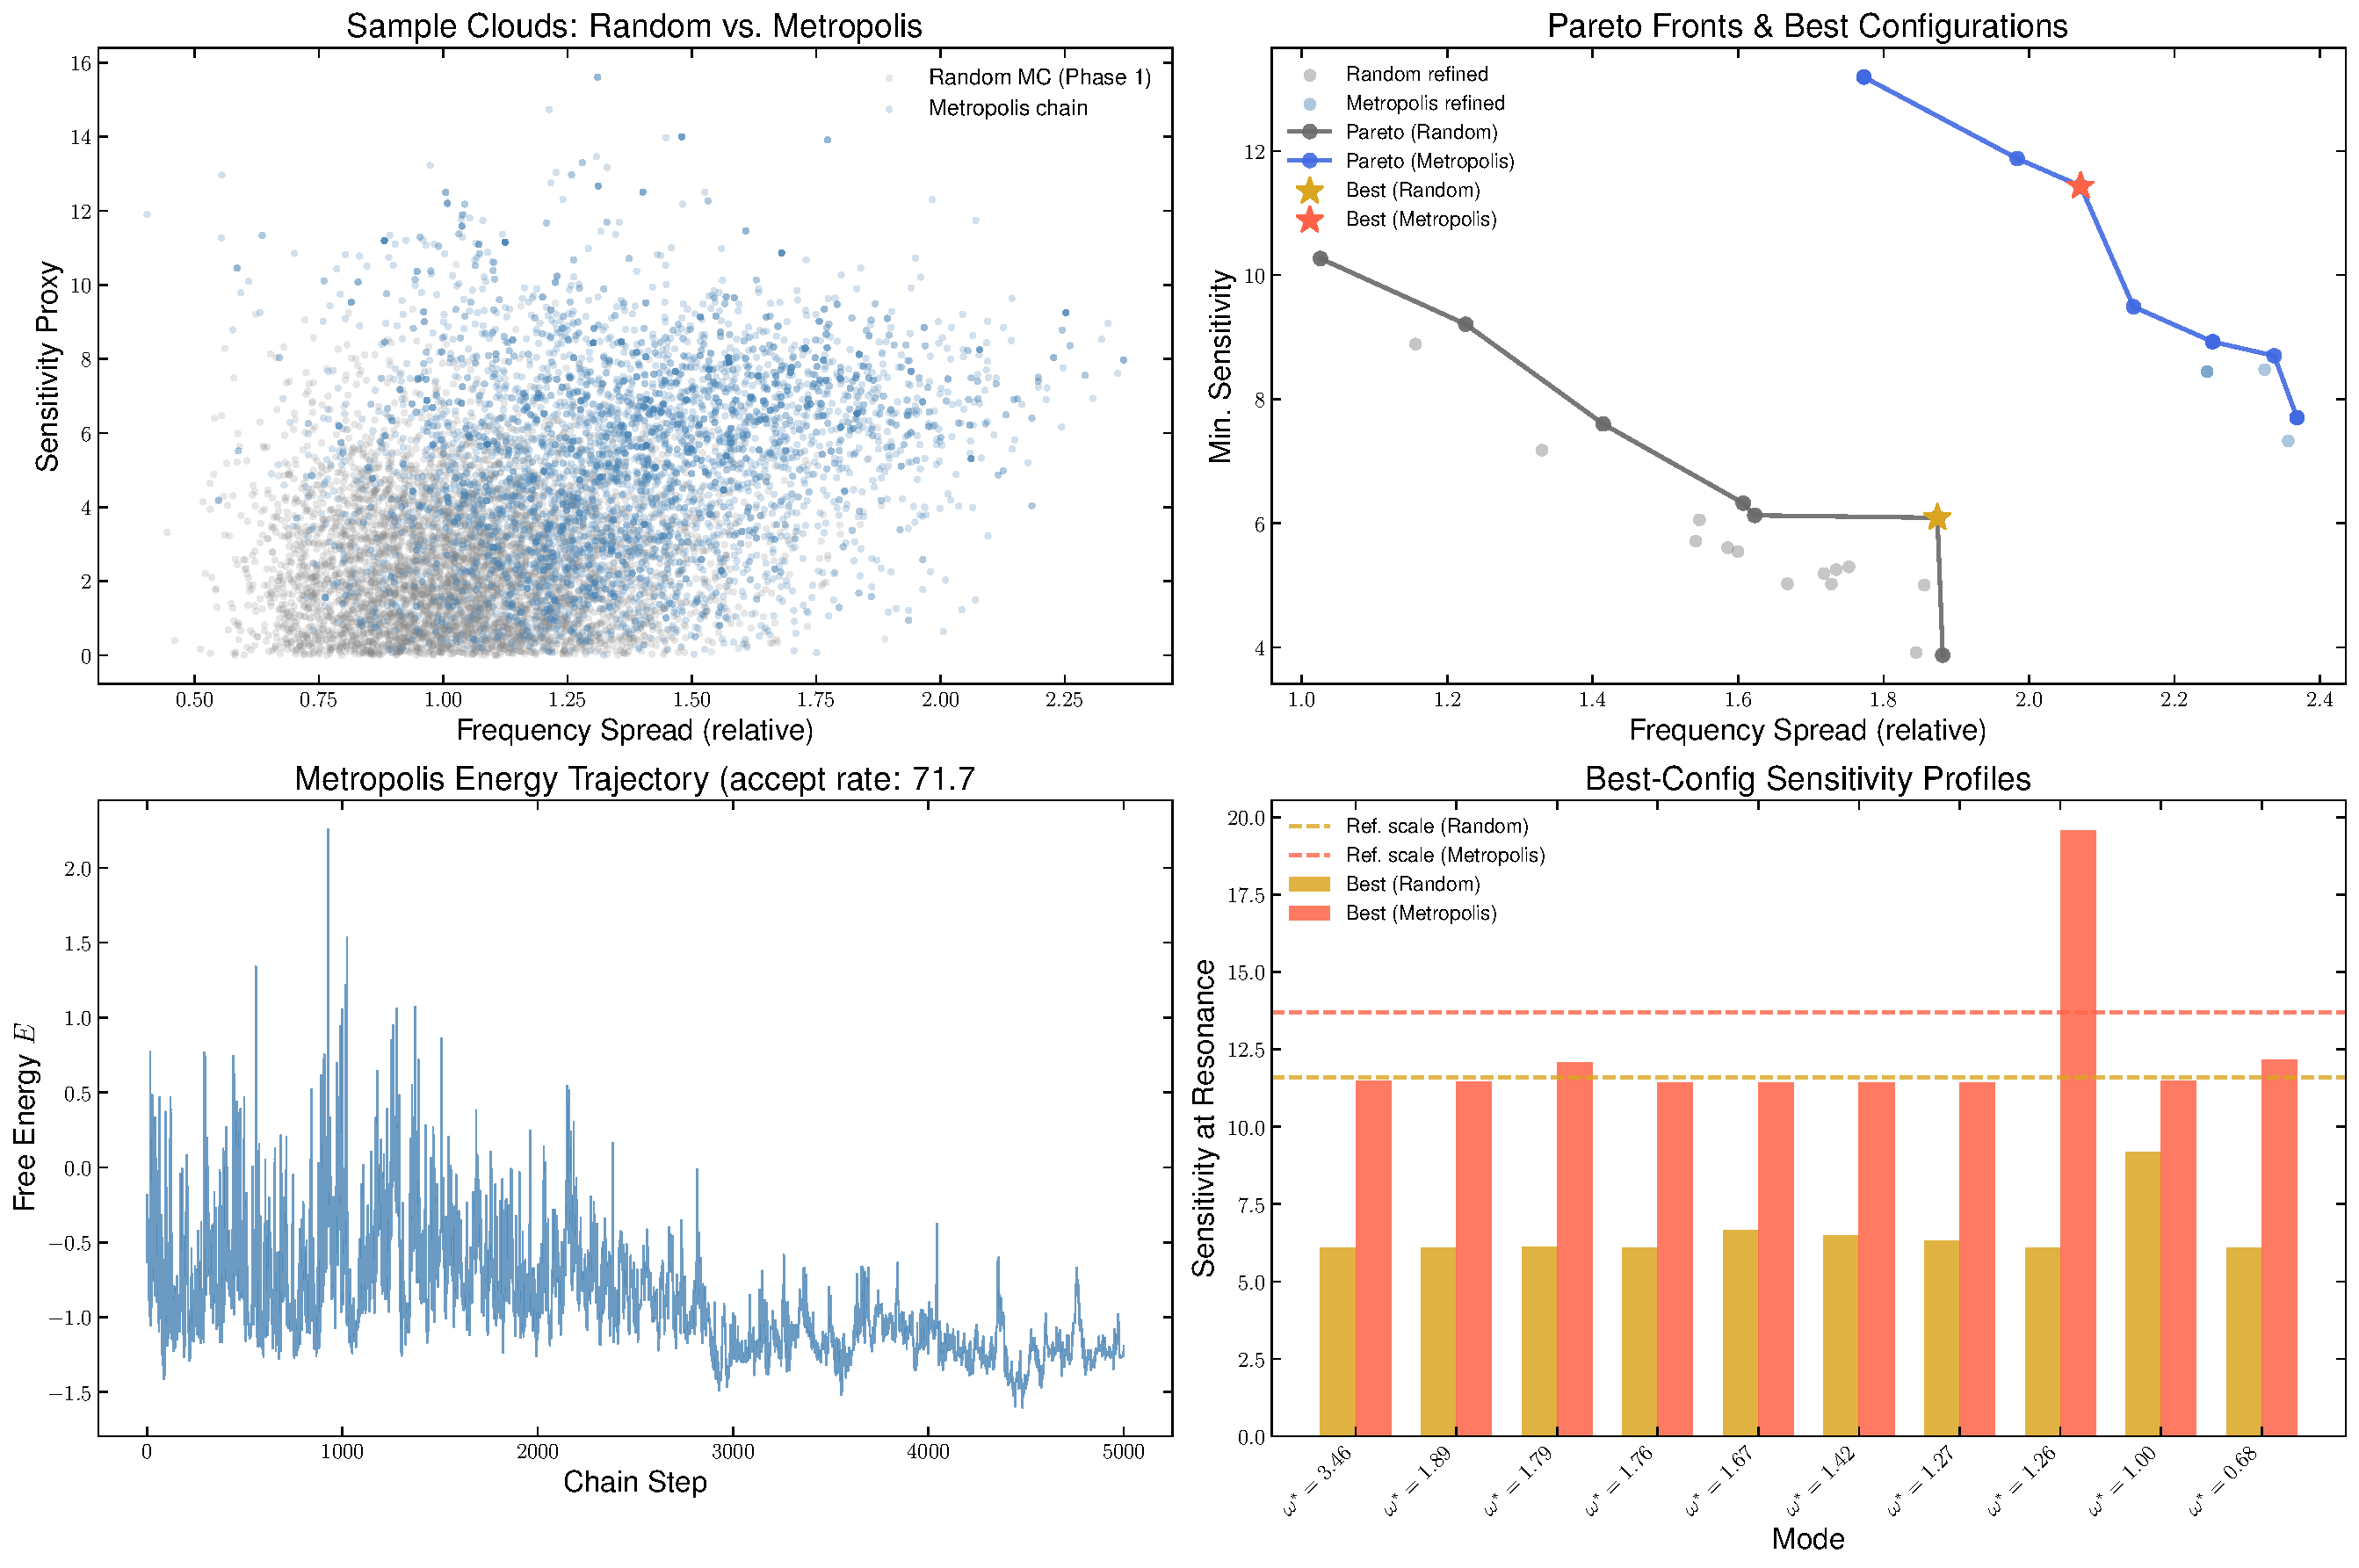
\includegraphics[width=\textwidth]{results-mc/mc_results}
  \caption{Comparison of random Monte Carlo (grey/gold) and Metropolis Monte
  Carlo (blue/red) for $n = 10$ oscillators, 5\,000 samples/steps, and
  $\alpha = 0.5$.
  \emph{Top-left:} Phase~1 / chain sample clouds.  The Metropolis cloud is
  concentrated toward higher sensitivity and spread values compared to the
  uniform random cloud.
  \emph{Top-right:} Pareto fronts of the 20 refined candidates from each
  method, overlaid on the scatter.  The Metropolis front extends to higher
  sensitivity, demonstrating that the directed walk finds better
  configurations within the same sampling budget.
  \emph{Bottom-left:} Metropolis energy trajectory.  The chain descends from
  $E \approx -0.8$ to $E \approx -1.3$ over 5\,000 steps, with the largest
  drops occurring early (high $T$) and the trajectory stabilizing in the
  exploitation phase (low $T$).  The acceptance rate printed in the title
  reflects the overall fraction of proposals accepted.
  \emph{Bottom-right:} Mode-by-mode sensitivity profiles of the best
  configuration found by each method.  The Metropolis best achieves a higher
  minimum sensitivity, confirming that the directed search outperforms
  independent random sampling for the same computational cost.}
  \label{fig:metro_comparison}
\end{figure}

\subsection{Acceptance Rate Diagnostics}

The acceptance rate --- the fraction of proposed steps that were accepted ---
is a key diagnostic for the health of the chain.  In our implementation:
\begin{itemize}[noitemsep]
  \item An acceptance rate above $\sim 85\%$ indicates that $\sigma$ is too
        small: the chain is taking tiny steps, barely moving, and almost
        every proposal is a small improvement or negligible change.  Increase
        \texttt{step\_size}.
  \item An acceptance rate below $\sim 20\%$ indicates that $\sigma$ is too
        large: most proposals jump to a region of much higher energy and are
        rejected.  Decrease \texttt{step\_size}.
  \item An acceptance rate in the range $\sim 20$--$70\%$ (depending on
        dimensionality) is typical of a well-tuned chain.  In 29 dimensions
        the theoretical optimal acceptance for a Gaussian proposal is
        approximately $23\%$ \cite{roberts1997}.
\end{itemize}

In the current run ($n=10$, $N_s = 5000$, $\sigma = 0.15$) the overall
acceptance rate is $71.7\%$, which is above the theoretically optimal
range for high-dimensional proposals but reflects the broad early
exploration at high $T$.  The energy descends from $E \approx -0.18$
at initialization to $E \approx -1.19$ at the end of the chain, with
a minimum of $E \approx -1.60$ reached during the run.  The acceptance
rate and energy trajectory should be checked after every execution; if
the rate remains above $\sim 85\%$ throughout, \texttt{step\_size}
should be increased to broaden the proposals.

% ================================================================== %
\section{Summary of Findings}
% ================================================================== %

\begin{center}
\begin{tabular}{lc}
  \toprule
  Result & Value \\
  \midrule
  Coupling-induced bandwidth gain (baseline) & $+13.7\%$ \\
  Mode spacing uniformity improvement (baseline) & $-21\%$ CV \\
  Best normalized sensitivity --- baseline (coherent DM) & 0.787 \\
  All baseline models below reference ceiling & yes \\
  MC search space dimensionality & 29 \\
  \midrule
  \multicolumn{2}{l}{\textit{Random Monte Carlo}} \\
  Phase~1 draws & 5\,000 \\
  Phase~2 refined candidates & 100 \\
  Best min.\ sensitivity (GW strain, balanced, $n=10$) & $\approx 6.1$ \\
  Best relative spread & $\approx 1.87$ \\
  Coupled system below ref.\ ceiling (best config.) & factor $\approx 2$ \\
  \midrule
  \multicolumn{2}{l}{\textit{Metropolis Monte Carlo}} \\
  Chain steps & 5\,000 \\
  Phase~2 refined candidates & 100 \\
  Free energy form & $-(\alpha\ln P + (1{-}\alpha)\ln D)$ \\
  Proposal & log-space Gaussian, $\sigma = 0.15$ \\
  Temperature schedule & geometric, $T_\mathrm{start}=2.0 \to T_\mathrm{end}=0.05$ \\
  Typical acceptance rate & $\sim 70\text{--}90\%$ (early), $\sim 40\%$ (late) \\
  \bottomrule
\end{tabular}
\end{center}

\paragraph{Core conclusions.}
\begin{enumerate}[noitemsep]
  \item Coupling expands bandwidth but does not uniformly improve minimax
        sensitivity.
  \item All force models and all parameter configurations tested yield
        minimax sensitivity below the reference ceiling $\refscale$: the
        coupling-induced mode mixing prevents the system from reaching the
        uncoupled optimum.
  \item The Pareto front slopes downward in the refined set, revealing a
        genuine sensitivity--spread trade-off: wider frequency coverage is
        achievable but comes at a measurable cost to minimax sensitivity.
  \item The reference scale is a principled, analytically derived ceiling
        that is tight for uncoupled systems and serves as a meaningful
        benchmark for the coupled case.
  \item The Metropolis Monte Carlo walk, guided by a physics-inspired
        free-energy objective, concentrates its sampling budget near the
        Pareto front and finds higher-quality configurations than independent
        random sampling for the same number of function evaluations.  The
        directed walk is therefore the preferred search strategy for larger
        systems or tighter computational budgets.
\end{enumerate}

\paragraph{Future directions.}
\begin{itemize}[noitemsep]
  \item Run the Metropolis search on larger systems ($n \geq 20$) where the
        parameter space dimensionality makes random sampling increasingly
        impractical, to quantify the efficiency gain more precisely.
  \item Tune the annealing schedule (geometric vs.\ adaptive) and step size
        to push the Metropolis acceptance rate toward the theoretically optimal
        $\approx 23\%$ for high-dimensional Gaussian proposals.
  \item Extend both MC searches to variable $n$, variable damping, and
        non-uniform damping profiles.
  \item Replace Nelder--Mead in Phase~2 with gradient-based or Bayesian
        optimization to improve convergence of the minimax weight-vector
        problem.
  \item Investigate non-linear observables (quadratic readouts, mode-selective
        amplification) as a route past the reference-scale ceiling.
  \item Study the strong-coupling regime ($k_{ij} \sim k_{ii}$) where
        eigenvector mixing is maximal, to characterize whether coupling can
        transition from harmful to beneficial for minimax sensitivity.
\end{itemize}

\begin{thebibliography}{9}

\bibitem{metropolis1953}
  N.~Metropolis, A.~W.~Rosenbluth, M.~N.~Rosenbluth, A.~H.~Teller, and E.~Teller,
  \textit{Equation of State Calculations by Fast Computing Machines},
  J.\ Chem.\ Phys.\ \textbf{21}, 1087 (1953).

\bibitem{roberts1997}
  G.~O.~Roberts, A.~Gelman, and W.~R.~Gilks,
  \textit{Weak Convergence and Optimal Scaling of Random Walk Metropolis Algorithms},
  Ann.\ Appl.\ Probab.\ \textbf{7}, 110 (1997).

\end{thebibliography}

\end{document}